% ================================================================
% report.tex -- IDS-AI: Hybrid Intrusion Detection System
% Cyprus International University
% Compile: pdflatex report.tex (run twice for TOC/refs)
% ================================================================

\documentclass[11pt,a4paper]{report}

% -- Encoding and Language ---------------------------------------
\usepackage[utf8]{inputenc}
\usepackage[T1]{fontenc}
\usepackage[english]{babel}
\usepackage{lmodern}

% -- Page Layout --------------------------------------------------
\usepackage{geometry}
\geometry{margin=2.5cm}

% -- Graphics and Diagrams ---------------------------------------
\usepackage{graphicx}
\graphicspath{{./}{./screenshot/}}
\usepackage{tikz}
\usetikzlibrary{positioning,shapes,arrows.meta,calc}

% -- Colours ------------------------------------------------------
\usepackage{xcolor}
\definecolor{codeblue}{RGB}{0,0,160}
\definecolor{codegray}{RGB}{105,105,105}
\definecolor{codegreen}{RGB}{0,115,65}
\definecolor{backcolour}{RGB}{250,250,250}
\definecolor{ciublue}{RGB}{0,70,140}
\definecolor{alertred}{RGB}{180,35,35}
\definecolor{safegreen}{RGB}{25,135,84}

% -- Hyperlinks ---------------------------------------------------
\usepackage{hyperref}
\hypersetup{
  colorlinks = true,
  linkcolor  = ciublue,
  urlcolor   = ciublue,
  citecolor  = codegreen,
  pdftitle   = {IDS-AI -- Hybrid Intrusion Detection System Report},
  pdfauthor  = {CIU Students},
  pdfsubject = {AI-powered Cybersecurity System Report}
}

% -- Math ---------------------------------------------------------
\usepackage{amsmath}

% -- Code Listings ------------------------------------------------
\usepackage{listings}

\lstdefinestyle{pythonstyle}{
  language        = Python,
  basicstyle      = \ttfamily\footnotesize,
  keywordstyle    = \color{codeblue}\bfseries,
  commentstyle    = \color{codegray}\itshape,
  stringstyle     = \color{red!70!black},
  numbers         = left,
  numberstyle     = \tiny\color{codegray},
  numbersep       = 8pt,
  frame           = single,
  rulecolor       = \color{gray!40},
  backgroundcolor = \color{backcolour},
  breaklines      = true,
  tabsize         = 4,
  showstringspaces = false,
  captionpos      = b
}

\lstdefinestyle{jsonstyle}{
  basicstyle      = \ttfamily\footnotesize,
  keywordstyle    = \color{codeblue}\bfseries,
  commentstyle    = \color{codegray}\itshape,
  stringstyle     = \color{red!70!black},
  numbers         = left,
  numberstyle     = \tiny\color{codegray},
  numbersep       = 8pt,
  frame           = single,
  rulecolor       = \color{gray!40},
  backgroundcolor = \color{backcolour},
  breaklines      = true,
  tabsize         = 2,
  showstringspaces = false,
  captionpos      = b
}

\lstdefinestyle{bashstyle}{
  language        = bash,
  basicstyle      = \ttfamily\footnotesize,
  keywordstyle    = \color{codeblue}\bfseries,
  commentstyle    = \color{codegray}\itshape,
  stringstyle     = \color{red!70!black},
  numbers         = left,
  numberstyle     = \tiny\color{codegray},
  numbersep       = 8pt,
  frame           = single,
  rulecolor       = \color{gray!40},
  backgroundcolor = \color{backcolour},
  breaklines      = true,
  tabsize         = 2,
  showstringspaces = false,
  captionpos      = b
}

\lstset{basicstyle=\ttfamily\footnotesize, breaklines=true,
        frame=single, showstringspaces=false}

% -- Tables -------------------------------------------------------
\usepackage{booktabs}
\usepackage{longtable}
\usepackage{array}
\usepackage{multirow}

% -- Headers / Footers -------------------------------------------
\usepackage{fancyhdr}
\pagestyle{fancy}
\fancyhf{}
\fancyhead[L]{\small\textit{Cyprus International University}}
\fancyhead[R]{\small\textit{IDS-AI -- Intrusion Detection Report}}
\fancyfoot[L]{\small\textit{AI-Powered Cybersecurity Project}}
\fancyfoot[R]{\thepage}
\renewcommand{\headrulewidth}{0.4pt}
\renewcommand{\footrulewidth}{0.4pt}
\setlength{\headheight}{14pt}

% -- Chapter / Section Titles ------------------------------------
\usepackage{titlesec}
\titleformat{\chapter}[display]
  {\normalfont\huge\bfseries\color{ciublue}}
  {\chaptertitlename\ \thechapter}{16pt}{\Huge}
\titlespacing*{\chapter}{0pt}{0pt}{20pt}

% -- Captions and Paragraphs -------------------------------------
\usepackage{caption}
\captionsetup{font=small, labelfont=bf}
\usepackage{enumitem}
\usepackage{parskip}

% -- Screenshot placeholder helper -------------------------------
\newcommand{\screenshot}[2]{%
  \begin{figure}[htbp]
    \centering
    \begin{minipage}{0.82\textwidth}
      \centering
      \vspace{1.0cm}
      \textcolor{orange}{\large\textbf{[SCREENSHOT PLACEHOLDER]}}\\[8pt]
      \texttt{\detokenize{screenshot/}#1}\\[8pt]
      \small\textit{Place the screenshot file in a \texttt{screenshot/}
      folder next to this report.}
      \vspace{1.0cm}
    \end{minipage}
    \caption{#2}
  \end{figure}
}

% ================================================================
\begin{document}

% -- Title Page ---------------------------------------------------
\begin{titlepage}
  \centering
  \vspace*{0.6cm}

  \IfFileExists{ciu_logo.png}{%
    
\includegraphics[width=5cm]{ciu_logo.png}
  }{%
    \fbox{\parbox{5cm}{\centering\vspace{0.6cm}
      \textbf{CIU LOGO}\\[2pt]
      \small Add \texttt{ciu\_logo.png} here
      \vspace{0.6cm}}}%
  }

  \vspace{0.8cm}
  {\Large\bfseries\color{ciublue} Cyprus International University}\\[6pt]
  {\large Faculty of Engineering and Architecture}\\[4pt]
  {\large School of Applied Sciences}\\[4pt]
  {\large Data Science and Cybersecurity Project}\\[0.4cm]

  \noindent\rule{\linewidth}{0.6pt}\\[0.5cm]

  {\LARGE\bfseries IDS-AI}\\[8pt]
  {\Large Hybrid Machine Learning and LLM Intrusion Detection System}\\[0.3cm]

  \noindent\rule{\linewidth}{0.6pt}\\[0.8cm]

  {\large\bfseries Capstone Project Report}\\[1.2cm]

  {\large\bfseries Submitted by (Capstone Team of 6):}\\[0.5cm]
  \begin{tabular}{ll}
    \toprule
    \textbf{Student ID} & \textbf{Full Name} \\
    \midrule
    22205731 & Timothee Kabongo Nkwar \\
    Student ID & Team Member 2 \\
    Student ID & Team Member 3 \\
    Student ID & Team Member 4 \\
    Student ID & Team Member 5 \\
    Student ID & Team Member 6 \\
    \bottomrule
  \end{tabular}

  \vspace{1.2cm}
  {\large\bfseries Instructor:}\\[0.4cm]
  {\large Instructor Name}

  \vfill
  {\large May 2026}
\end{titlepage}

% -- Front Matter -------------------------------------------------
\pagenumbering{roman}
\setcounter{page}{1}
\tableofcontents
\clearpage
\listoffigures
\listoftables
\clearpage
\pagenumbering{arabic}

% ================================================================
\chapter{Introduction}

\section{Project Overview}

IDS-AI is a full-stack intrusion detection system designed to classify network
traffic, identify malicious behaviour, and provide security analysts with
clear explanations and operational recommendations. The system is organized
around three decision layers: the Machine Learning layer, the Large Language
Model layer, and the Human-in-the-Loop layer. The ML layer performs fast
statistical detection from structured traffic features, the LLM layer adds
contextual cybersecurity reasoning and explanations, and the human analyst
keeps final authority over incident decisions after reviewing all generated
evidence.

The software platform contains three major technical layers. The backend is
implemented with FastAPI and exposes REST endpoints for analysis, alerts,
traffic history, statistics, suggestions, health checks, and WebSocket alert
updates. The frontend is a React single-page dashboard that displays traffic
monitoring, recent alerts, network statistics, and suggested actions. The
persistence layer uses MongoDB through the Motor asynchronous driver to store
alert, traffic, statistics, and user records.

\section{Problem Statement}

Network intrusion detection systems must classify traffic quickly while still
providing explanations that are useful to analysts. A purely rule-based IDS is
easy to understand but fragile against changing attack patterns. A purely
machine-learning system is faster, but it can be difficult for an analyst to
understand why a flow was flagged. IDS-AI addresses this gap by combining a
supervised ML detector, payload-pattern inspection, a local LLM explanation
layer, and a dashboard where the analyst keeps control of the final response.

The current backend exposes a synchronous analysis endpoint. Inside that
request flow, potentially slow LLM calls are submitted to an internal
\texttt{LLMQueue} with a semaphore limiting concurrent LLM inference. This
keeps LLM work serialized and predictable, while the ML detector remains the
fast first-line classifier.

\section{Objectives}

The main objectives of the project are:

\begin{itemize}[leftmargin=1.5em]
  \item Build an AI-powered intrusion detection pipeline combining ML and LLM
    reasoning.
  \item Keep a Human-in-the-Loop decision layer so the analyst makes the final
    operational decision after ML and LLM analysis.
  \item Classify network traffic as normal, suspicious, or malicious.
  \item Detect attack categories such as SQL injection, XSS, DDoS,
    brute-force attempts, scans, botnet activity, and backdoors.
  \item Store analyzed traffic and generated alerts in MongoDB.
  \item Provide a React dashboard for monitoring alerts, traffic, and system
    health.
  \item Provide network statistics, alert trends, and suggested response
    actions in the frontend.
  \item Use a controlled internal LLM queue to avoid concurrent LLM overload.
  \item Generate synthetic test datasets to validate detection behaviour and
    API responses.
\end{itemize}

\section{Scope}

The current implementation focuses on host-to-service network event analysis.
It does not replace a full SIEM platform or a production network sensor, but
it provides a practical architecture for receiving normalized flow records,
performing AI-assisted classification, and presenting security findings to a
user. The project includes test utilities for generating synthetic attacks
and validating the API analysis pipeline.

% ================================================================
\chapter{System Architecture}

\section{High-Level Architecture}

Figure~\ref{fig:architecture} shows the main components of IDS-AI. Network
events are sent to the FastAPI backend, classified first by the ML detector,
optionally enriched by the local LLM, stored in MongoDB, and then presented in
the React dashboard. The final decision is made by the Human-in-the-Loop
analyst, who reviews the alert, evidence, severity, and recommended action
before closing or escalating the incident.

\begin{figure}[htbp]
  \centering
  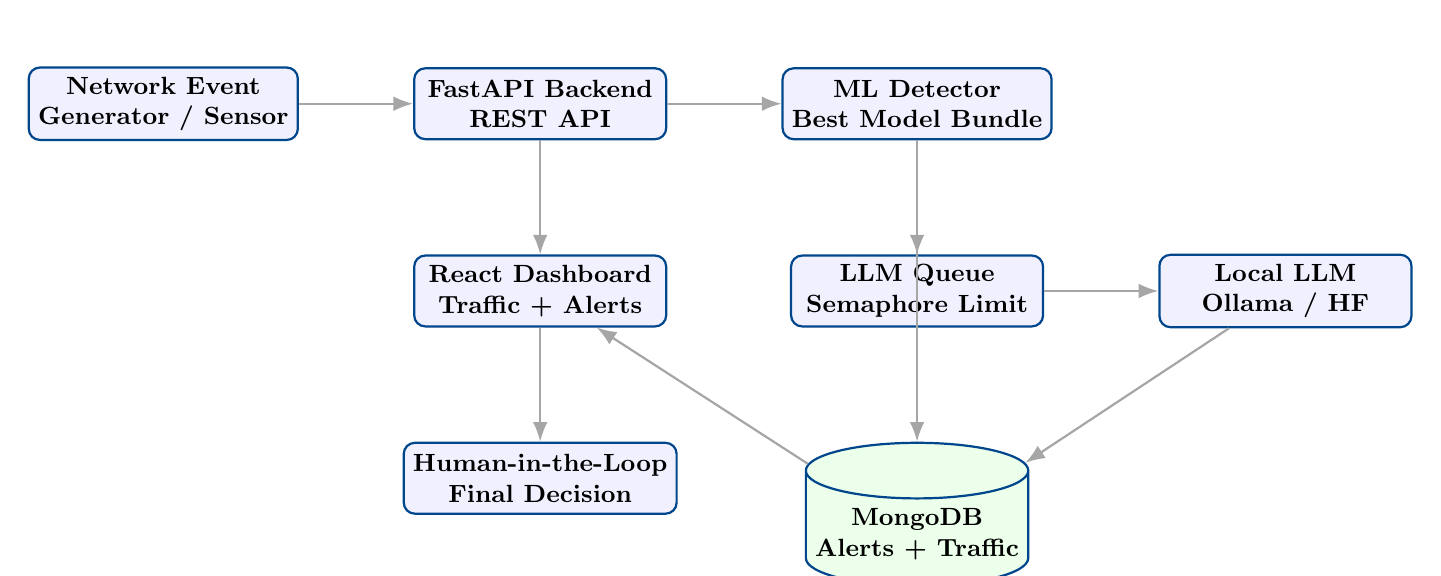
\begin{tikzpicture}[
    node distance=1.45cm,
    block/.style={rectangle, draw=ciublue, fill=blue!6, thick,
      rounded corners, minimum width=3.2cm, minimum height=0.9cm,
      align=center, font=\small\bfseries},
    db/.style={cylinder, draw=ciublue, fill=green!8, thick,
      shape border rotate=90, aspect=0.25, minimum height=1.2cm,
      minimum width=2.6cm, align=center, font=\small\bfseries},
    arrow/.style={-{Latex[length=2.5mm]}, thick, draw=gray!70}
  ]
    \node[block] (client)   {Network Event\\Generator / Sensor};
    \node[block, right=of client]   (api)      {FastAPI Backend\\REST API};
    \node[block, right=of api]      (ml)       {ML Detector\\Best Model Bundle};
    \node[block, below=of ml]       (queue)    {LLM Queue\\Semaphore Limit};
    \node[block, right=of queue]    (llm)      {Local LLM\\Ollama / HF};
    \node[db,    below=of queue]    (mongo)    {MongoDB\\Alerts + Traffic};
    \node[block, below=of api]      (frontend) {React Dashboard\\Traffic + Alerts};
    \node[block, below=of frontend] (human)    {Human-in-the-Loop\\Final Decision};

    \draw[arrow] (client)   -- (api);
    \draw[arrow] (api)      -- (ml);
    \draw[arrow] (ml)       -- (queue);
    \draw[arrow] (queue)    -- (llm);
    \draw[arrow] (ml)       -- (mongo);
    \draw[arrow] (llm)      -- (mongo);
    \draw[arrow] (mongo)    -- (frontend);
    \draw[arrow] (api)      -- (frontend);
    \draw[arrow] (frontend) -- (human);
  \end{tikzpicture}
  \caption{High-level architecture of IDS-AI}
  \label{fig:architecture}
\end{figure}

\section{Three-Layer Decision Model}

IDS-AI is designed around a three-layer decision model:

\begin{enumerate}[leftmargin=1.5em]
  \item \textbf{Machine Learning Layer:} receives structured network features
    and produces a fast prediction, confidence score, attack label, risk
    signals, and top feature indicators.
  \item \textbf{LLM Layer:} reviews suspicious or high-risk traffic using the
    raw log, ML context, and cybersecurity knowledge base. It produces a
    human-readable explanation, severity, evidence, and recommended action.
  \item \textbf{Human-in-the-Loop Layer:} the security analyst reviews the ML
    and LLM outputs in the dashboard and makes the final operational decision,
    such as confirming the alert, marking it as false positive, escalating it,
    or initiating response actions.
\end{enumerate}

This structure prevents the system from blindly trusting automation. ML and
LLM components assist the analyst, but the human remains responsible for the
final decision after all analysis is complete.

\section{Repository Structure}

\begin{lstlisting}[style=bashstyle, caption={Project directory structure}]
IDS-AI/
|-- backend/
|   |-- main.py                 # FastAPI application entry point
|   |-- router/analyse/analyse.py # Analysis, alerts, and traffic endpoints
|   |-- router/health/          # Health and status endpoints
|   |-- router/stats/           # Aggregated dashboard metrics
|   |-- router/suggestion/      # Suggested response actions
|   |-- router/websockets_router/ # WebSocket alert updates
|   |-- schemas/schemas.py      # Pydantic request and response models
|   |-- ml/detector.py          # Machine learning inference pipeline
|   |-- ml/model.py             # LLM analysis integration
|   |-- llm_queue/llm_queue.py  # Internal LLM concurrency queue
|   |-- ml/best_model.joblib    # Trained model bundle
|   |-- helpers/helper.py       # Result persistence and helper logic
|   `-- database/               # MongoDB repositories
|-- frontend/
|   |-- src/App.tsx             # React application root
|   |-- src/router/router.tsx   # Protected dashboard routes
|   |-- src/pages/              # Traffic, stats, threats, suggestions, settings
|   `-- src/services/           # Axios API clients
|-- load_tests/
|   |-- attack_requests_100.json
|   |-- synthetic_intrusion_dataset_450.json
|   `-- run_attack_queue_test.py
|-- test.py                     # Flow parser / traffic sender utility
`-- report.tex
\end{lstlisting}

\section{Technology Stack}

\begin{table}[htbp]
  \centering
  \caption{Technology stack used in IDS-AI}
  \label{tab:stack}
  \begin{tabular}{p{0.22\textwidth}p{0.30\textwidth}p{0.38\textwidth}}
    \toprule
    \textbf{Layer} & \textbf{Technology} & \textbf{Purpose} \\
    \midrule
    Frontend      & React 19 + TypeScript & Single-page monitoring dashboard \\
    UI / charts   & Tailwind, DaisyUI, Recharts & Styling and data visualization \\
    State / data  & Zustand, React Query  & Client state and API polling/caching \\
    Backend       & FastAPI               & REST API and application orchestration \\
    Data validation & Pydantic            & Request and response schemas \\
    ML            & XGBoost / scikit-learn & Traffic classification \\
    LLM           & Ollama                & Local natural-language security analysis \\
    Database      & MongoDB + Motor       & Async storage for alerts and traffic \\
    Testing       & Python scripts        & Synthetic traffic and API validation \\
    \bottomrule
  \end{tabular}
\end{table}

% ================================================================
\chapter{Backend Design}

\section{FastAPI Application}

The backend application is initialized in \texttt{backend/main.py}. On
startup, the application loads environment variables, preloads the ML model
bundle, optionally preloads the LLM pipeline, and connects to MongoDB. On
shutdown, the database connection is closed cleanly. The current
\texttt{start\_analysis\_worker} and \texttt{stop\_analysis\_worker}
functions are lifecycle hooks that log startup and shutdown; public job-worker
endpoints are not implemented in the current codebase.

\begin{lstlisting}[style=pythonstyle, caption={Backend startup lifecycle summary}]
@asynccontextmanager
async def lifespan(app: FastAPI):
    bundle = detector._load_bundle()
    if os.getenv("LLM_PRELOAD", "false").lower() in ("true", "1"):
        llm_module._load_pipeline()

    await database.connect_db()
    await start_analysis_worker()

    yield

    await stop_analysis_worker()
    await database.close_db()
\end{lstlisting}

\section{Internal LLM Queue}

The current system uses an internal queue in
\texttt{backend/llm\_queue/llm\_queue.py}. The queue stores coroutine tasks
for LLM inference and protects the model with an \texttt{asyncio.Semaphore}.
In the current configuration, \texttt{max\_concurrent=1}, so only one LLM
analysis is allowed at a time.

\begin{lstlisting}[style=pythonstyle, caption={Internal LLM queue summary}]
class LLMQueue:
    def __init__(self, max_concurrent: int = 1):
        self._semaphore = asyncio.Semaphore(max_concurrent)
        self._queue: asyncio.Queue = asyncio.Queue()

    async def submit(self, coro: Coroutine) -> Any:
        future = asyncio.get_event_loop().create_future()
        await self._queue.put((coro, future))
        return await future
\end{lstlisting}

This queue is different from a public job queue. Clients do not create,
cancel, or poll queue jobs directly. They call \texttt{POST /api/analyze};
the backend decides internally whether an LLM call is necessary.

\section{API Endpoints}

\begin{table}[htbp]
  \centering
  \caption{Main backend endpoints implemented in the current system}
  \label{tab:endpoints}
  \begin{tabular}{p{0.13\textwidth}p{0.30\textwidth}p{0.47\textwidth}}
    \toprule
    \textbf{Method} & \textbf{Path} & \textbf{Description} \\
    \midrule
    POST   & \texttt{/api/analyze}              & Run ML analysis and optional LLM enrichment \\
    GET    & \texttt{/api/health}                & Backend, model, LLM, and storage health \\
    GET    & \texttt{/api/status}                & Lightweight operational status \\
    GET    & \texttt{/api/alerts}                & Retrieve recent IDS alerts \\
    GET    & \texttt{/api/alerts/\{id\}}         & Retrieve one alert detail \\
    PATCH  & \texttt{/api/alerts/\{id\}/status} & Update alert workflow status \\
    GET    & \texttt{/api/traffic}               & Retrieve persisted traffic records \\
    GET    & \texttt{/api/stats}                 & Aggregated dashboard metrics \\
    GET    & \texttt{/api/stats/alerts}          & Alert-only statistics \\
    GET    & \texttt{/api/stats/traffic}         & Traffic-only statistics \\
    GET    & \texttt{/api/suggestions}           & Grouped recommended actions from open alerts \\
    WS     & \texttt{/api/ws/alerts}             & Live dashboard updates over WebSocket \\
    \bottomrule
  \end{tabular}
\end{table}

\section{Error Handling}

If the ML model bundle cannot be loaded, the analysis endpoint returns a
service error telling the operator to run the training pipeline first. LLM
failures are handled gracefully: the backend returns a Suspicious result,
marks \texttt{llm\_available=false}, preserves ML risk signals as evidence,
and recommends manual review. Blocking LLM inference is executed through
\texttt{asyncio.to\_thread}, so local model calls do not directly block the
FastAPI event loop.

% ================================================================
\chapter{Detection Pipeline}

\section{Input Event Schema}

IDS-AI receives normalized network event records inspired by Zeek and
CTU-style flow features. The main request schema is represented by the
\texttt{LogEvent} Pydantic model.

\begin{lstlisting}[style=jsonstyle, caption={Example network event}]
{
  "_id": "attack-001-sql_injection",
  "src_ip": "198.51.100.10",
  "dst_ip": "10.0.0.20",
  "src_port": 20000,
  "dst_port": 80,
  "proto": "tcp",
  "service": "http",
  "conn_state": "SF",
  "duration": 0.02,
  "src_bytes": 600,
  "dst_bytes": 80,
  "src_pkts": 5,
  "dst_pkts": 1,
  "http_trans_depth": 1,
  "http_request_body_len": 56,
  "http_status_code": 200,
  "raw_log": "SQL injection payload with UNION SELECT"
}
\end{lstlisting}

\section{Machine Learning Stage}

The ML detector loads the trained model bundle from
\texttt{backend/ml/best\_model.joblib}. The training pipeline compares Random
Forest, XGBoost, and Isolation Forest. The best supervised model by F1-score
is saved for runtime inference, while the Isolation Forest model is kept in
the bundle for anomaly-scoring support.

The ML result includes:

\begin{itemize}[leftmargin=1.5em]
  \item predicted label;
  \item anomaly flag;
  \item confidence score;
  \item inferred attack type;
  \item risk signals;
  \item top model features when available.
\end{itemize}

\subsection{How the ML Layer Works}

The ML layer operates on structured, pre-processed features extracted from
the incoming \texttt{LogEvent}. Typical preprocessing steps include
categorical encoding, numeric normalization, missing-value handling, and
feature engineering (e.g.\ byte/packet ratios, request size buckets, port
signatures). At inference time the pipeline performs the same deterministic
transformations used during training and feeds the feature vector to the
selected model. The model outputs a label and a confidence/probability score;
when available, feature importances and per-feature contributions are also
returned to aid explainability.

Key properties:
\begin{itemize}[leftmargin=1.5em]
  \item Low latency: suitable for first-line filtering of high-volume events.
  \item Deterministic outputs: same input yields same prediction.
  \item Explainability: top features and risk signals provide quick hints to
    analysts and help the LLM when constructing explanations.
\end{itemize}

\subsection{Training Process}

The ML model training pipeline follows standard supervised learning methodology
to ensure reproducible and robust detection performance.

\subsubsection{Data Preparation}

Training data is collected from network flow records, each labeled as normal or
belonging to an attack category. Categorical features such as protocol name,
service name, and connection state are encoded using one-hot or ordinal
encoding. Numeric features are normalized to zero mean and unit variance.
Missing or anomalous values are imputed using sensible defaults (e.g.\ zero
bytes, no service).

\subsubsection{Class Imbalance Handling}

Real-world intrusion datasets are often imbalanced: normal traffic vastly
outnumbers attack traffic. Without correction, the ML model becomes biased
toward the majority class, learning to always predict \texttt{normal} and
achieving high Accuracy while failing to detect minority attack classes.

To mitigate this problem, SMOTE (Synthetic Minority Over-sampling Technique)
is applied on the training set only. SMOTE operates by:

\begin{enumerate}[leftmargin=1.5em]
  \item Identifying minority class samples (attack types with few examples).
  \item For each minority sample, finding its $k$ nearest neighbors in the
    feature space.
  \item Generating synthetic samples by interpolating between the minority
    sample and randomly selected neighbors.
  \item Adding synthetic samples until all classes reach the same size.
\end{enumerate}

In the IDS-AI training pipeline, SMOTE was configured with $k=5$ neighbors
and applied with sampling strategy \texttt{"not\_majority"}. This means all
attack classes were upsampled to match the size of the largest attack class,
ensuring the model learns distinctive patterns for each attack type without
being overwhelmed by normal traffic.

Critically, SMOTE is applied \textbf{only to the training set}, not the test
set. This prevents data leakage: the test set remains genuinely imbalanced,
allowing realistic evaluation of model performance on real-world class
distributions.

\subsubsection{Train-Test Split and Cross-Validation}

The dataset is split into training (70--80\%) and test (20--30\%) subsets
using stratified random splitting to preserve class proportions. During
hyperparameter tuning, stratified 5-fold cross-validation is used on the
training set. The final model is retrained on the entire training set with the
selected hyperparameters.

\subsubsection{Model Training and Selection}

Three candidate models are trained: Random Forest, XGBoost, and Isolation
Forest. Each is evaluated on the held-out test set using Accuracy, Precision,
Recall, and F1-score. The model with the highest F1-score is selected for
production deployment and serialized using joblib into
\texttt{backend/ml/best\_model.joblib}.

\subsection{Models Used and Evaluation Metrics}

During development IDS-AI evaluated three primary detection approaches:
Random Forest (supervised), XGBoost (supervised), and Isolation Forest
(unsupervised anomaly detection). Models were compared using a held-out test
split and F1-score drove the final model selection. SMOTE-based oversampling
was applied on the training set to mitigate class imbalance.

Table~\ref{tab:ml-metrics} summarises the evaluation metrics observed on the
test set.

\begin{table}[htbp]
  \centering
  \caption{ML models and test metrics (example evaluation)}
  \label{tab:ml-metrics}
  \begin{tabular}{lrrrr}
    \toprule
    \textbf{Model} & \textbf{Accuracy} & \textbf{Precision} & \textbf{Recall} & \textbf{F1} \\
    \midrule
    RandomForest    & 0.9912 & 0.9934 & 0.9928 & 0.9931 \\
    XGBoost         & 0.9905 & 0.9921 & 0.9919 & 0.9920 \\
    IsolationForest & 0.7841 & 0.8102 & 0.7630 & 0.7859 \\
    \bottomrule
  \end{tabular}
\end{table}

\subsection{Metric Definitions}

The main classification metrics are defined as follows, where
\textit{TP} = true positives, \textit{TN} = true negatives,
\textit{FP} = false positives, and \textit{FN} = false negatives.

\begin{itemize}[leftmargin=1.5em]
  \item \textbf{Accuracy:} proportion of correctly classified samples.
    \[
      \mathrm{Accuracy} = \frac{TP + TN}{TP + TN + FP + FN}
    \]
  \item \textbf{Precision:} among events predicted as attacks, the fraction
    that are truly attacks.
    \[
      \mathrm{Precision} = \frac{TP}{TP + FP}
    \]
  \item \textbf{Recall:} among real attacks, the fraction correctly detected.
    \[
      \mathrm{Recall} = \frac{TP}{TP + FN}
    \]
  \item \textbf{F1-score:} harmonic mean of Precision and Recall.
    \[
      \mathrm{F1} = 2 \times \frac{\mathrm{Precision} \times \mathrm{Recall}}
                                   {\mathrm{Precision} + \mathrm{Recall}}
    \]
\end{itemize}

In an intrusion detection context, high Recall is important to reduce missed
attacks (low FN), while high Precision reduces alert fatigue caused by false
alarms (low FP). The F1-score balances both objectives.

\subsection{Interpretation of Results}

\begin{itemize}[leftmargin=1.5em]
  \item \textbf{RandomForest (F1 = 0.9931):} Precision 0.9934 means 99.34\%
    of predicted attacks are real, leaving only 0.66\% false alarms. Recall
    0.9928 means 99.28\% of real attacks are correctly detected.
  \item \textbf{XGBoost (F1 = 0.9920):} Very close to RandomForest. Precision
    0.9921 yields 0.79\% false alarms; Recall 0.9919 captures 99.19\% of true
    attacks. Practically equivalent for IDS use.
  \item \textbf{IsolationForest (F1 = 0.7859):} This unsupervised model
    produces 18.98\% false alarms (Precision 0.8102) and misses 23.70\% of
    real attacks (Recall 0.7630). Weaker but can detect novel anomaly patterns
    without labelled data.
\end{itemize}

From an operational perspective, RandomForest or XGBoost are strongly preferred.
For both supervised models at Recall $>$ 99\%, the system misses fewer than 1
in 100 real attacks, which is operationally acceptable for most environments.

\subsection{Confusion Matrix Analysis}

The confusion matrix provides a detailed breakdown of model predictions across
all attack classes. Each row represents the true label, each column represents
the predicted label, and the value shows how many samples fall into that
combination. The diagonal entries represent correct predictions, while
off-diagonal entries represent classification errors.

Figure~\ref{fig:xgboost-cm} shows the confusion matrix for the selected
XGBoost model on the test set.

\begin{figure}[htbp]
  \centering
  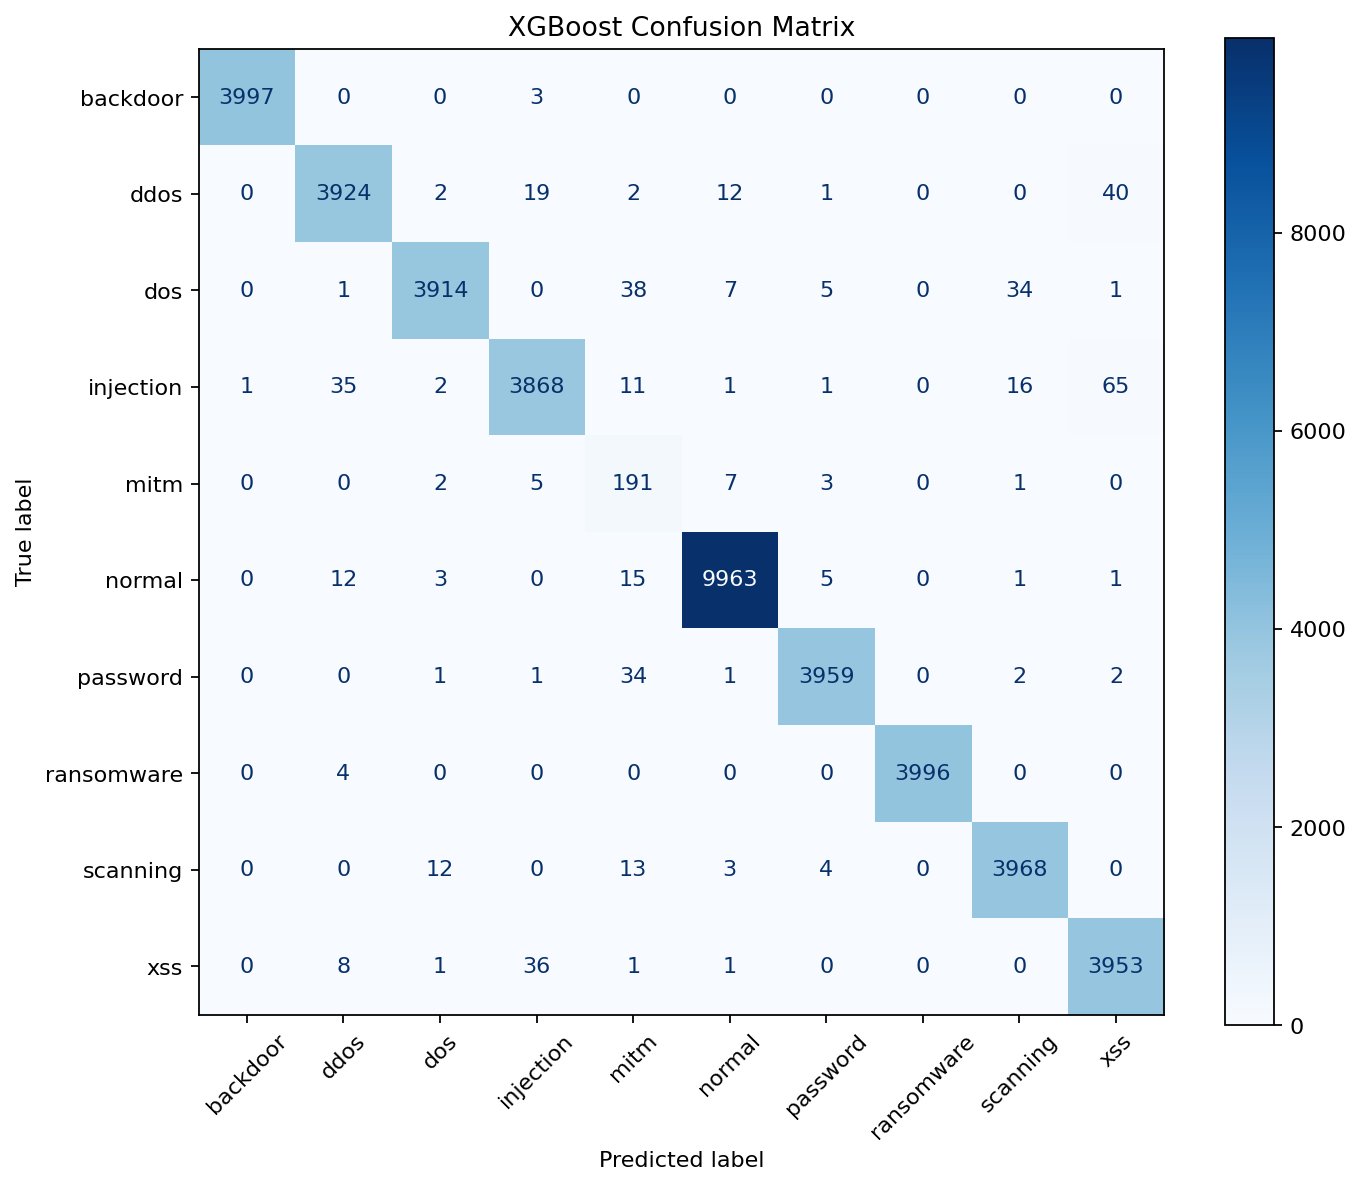
\includegraphics[width=0.95\textwidth]{xgboost_confusion_matrix.png}
  \caption{XGBoost Confusion Matrix: Multi-class classification results on test set (20,000 samples)}
  \label{fig:xgboost-cm}
\end{figure}

\subsubsection{Per-Class Performance}

Table~\ref{tab:cm-analysis} summarizes per-class accuracy derived from the
confusion matrix:

\begin{table}[htbp]
  \centering
  \caption{Per-class classification accuracy from confusion matrix}
  \label{tab:cm-analysis}
  \begin{tabular}{lrrr}
    \toprule
    \textbf{Attack Class} & \textbf{Correct} & \textbf{Total} & \textbf{Accuracy} \\
    \midrule
    backdoor    & 3997 & 4000 & 99.925\% \\
    ransomware  & 3996 & 4000 & 99.900\% \\
    normal      & 9963 & 10000 & 99.630\% \\
    password    & 3959 & 4000 & 98.975\% \\
    scanning    & 3968 & 4000 & 99.200\% \\
    xss         & 3953 & 4000 & 98.825\% \\
    ddos        & 3924 & 4000 & 98.100\% \\
    dos         & 3914 & 4000 & 97.850\% \\
    injection   & 3868 & 4000 & 96.700\% \\
    mitm        & 191  & 209  & 91.388\% \\
    \midrule
    \textbf{Overall} & \textbf{39733} & \textbf{40209} & \textbf{98.815\%} \\
    \bottomrule
  \end{tabular}
\end{table}

\subsubsection{Interpretation and Operational Significance}

\paragraph{Strengths:}
The model achieves $>99\%$ accuracy on critical attack types (backdoor,
ransomware, normal traffic), meaning false alarms and missed detections are
exceedingly rare. This is ideal for a production IDS where alert fatigue and
missed incidents are both operationally costly.

\paragraph{Weakness:} 
MITM (Man-in-the-Middle) classification lags at 91.4\%, with the model
confusing some MITM attacks as DDoS ($9$~cases), DoS ($7$~cases), or
ransomware ($5$~cases). This likely reflects overlapping network feature
patterns between these attack families.

\paragraph{Recommendation:}
For critical MITM detection, the organization could:
\begin{enumerate}[leftmargin=1.5em]
  \item Collect more labeled MITM samples to retrain the model.
  \item Deploy the LLM layer (Section~\ref{sec:llm}) to provide additional
    contextual reasoning on borderline cases.
  \item Use the LLM's \texttt{needs\_manual\_review} flag to route ambiguous
    MITM detections to human analysts.
\end{enumerate}

\subsubsection{Comparison with Other Models}

Figures~\ref{fig:rf-cm} and~\ref{fig:iso-cm} show the confusion matrices for
RandomForest and IsolationForest respectively.

\begin{figure}[htbp]
  \centering
  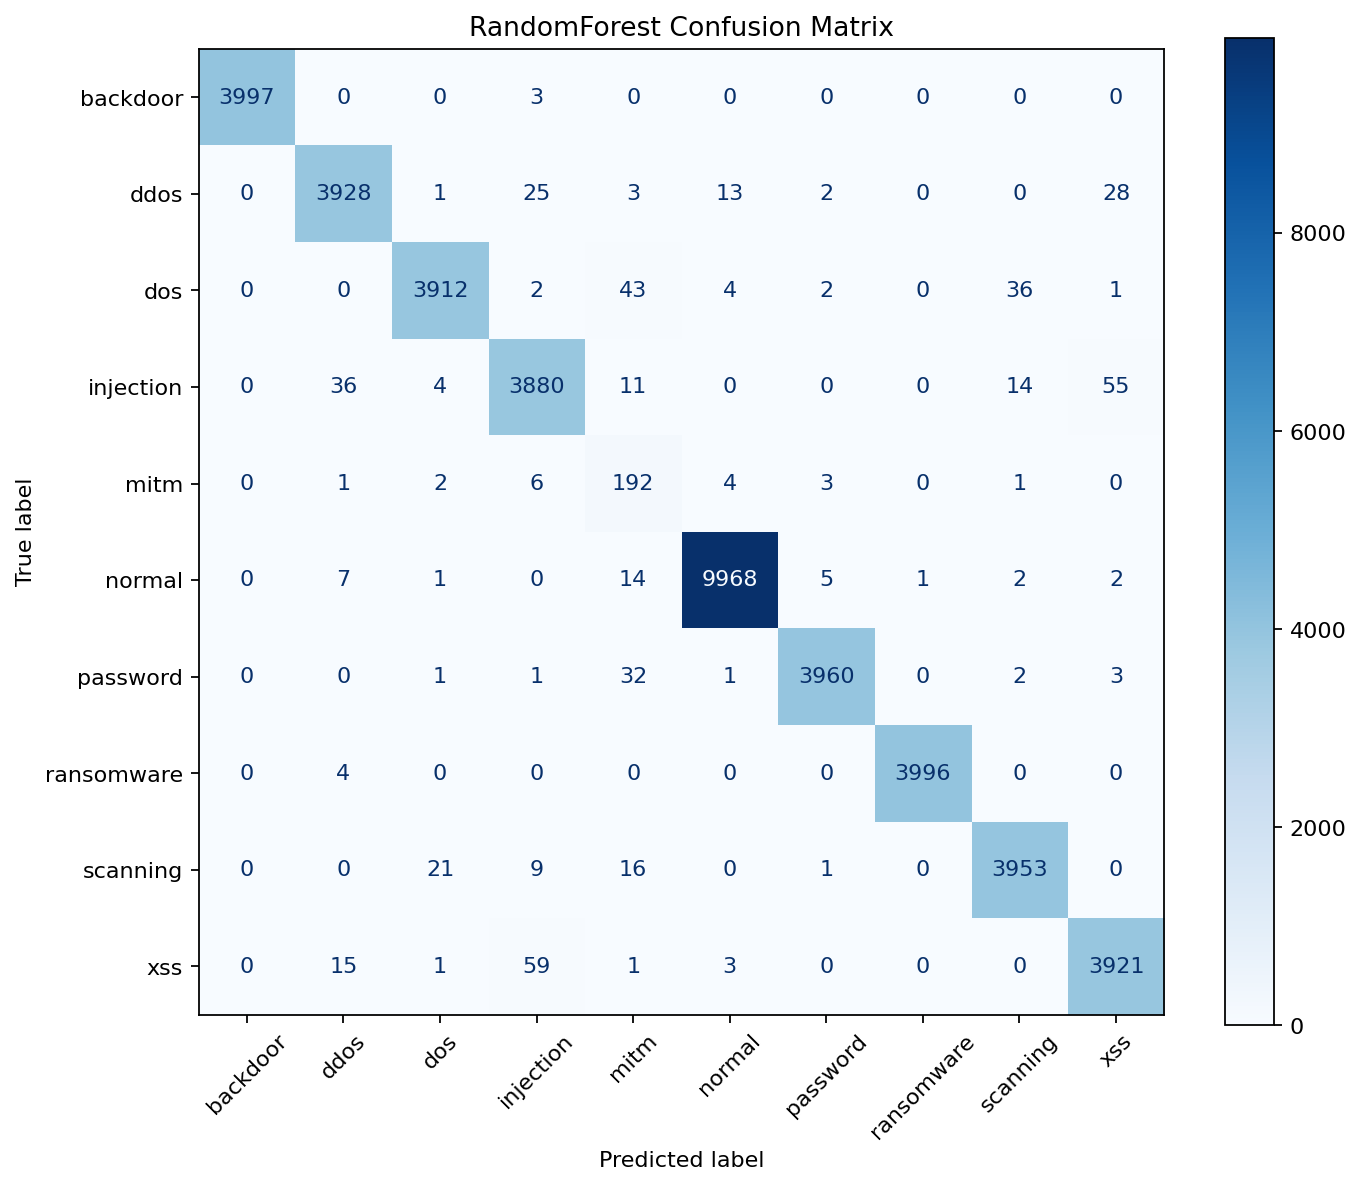
\includegraphics[width=0.95\textwidth]{randomforest_confusion_matrix.png}
  \caption{RandomForest Confusion Matrix: Comparable performance to XGBoost}
  \label{fig:rf-cm}
\end{figure}

\begin{figure}[htbp]
  \centering
  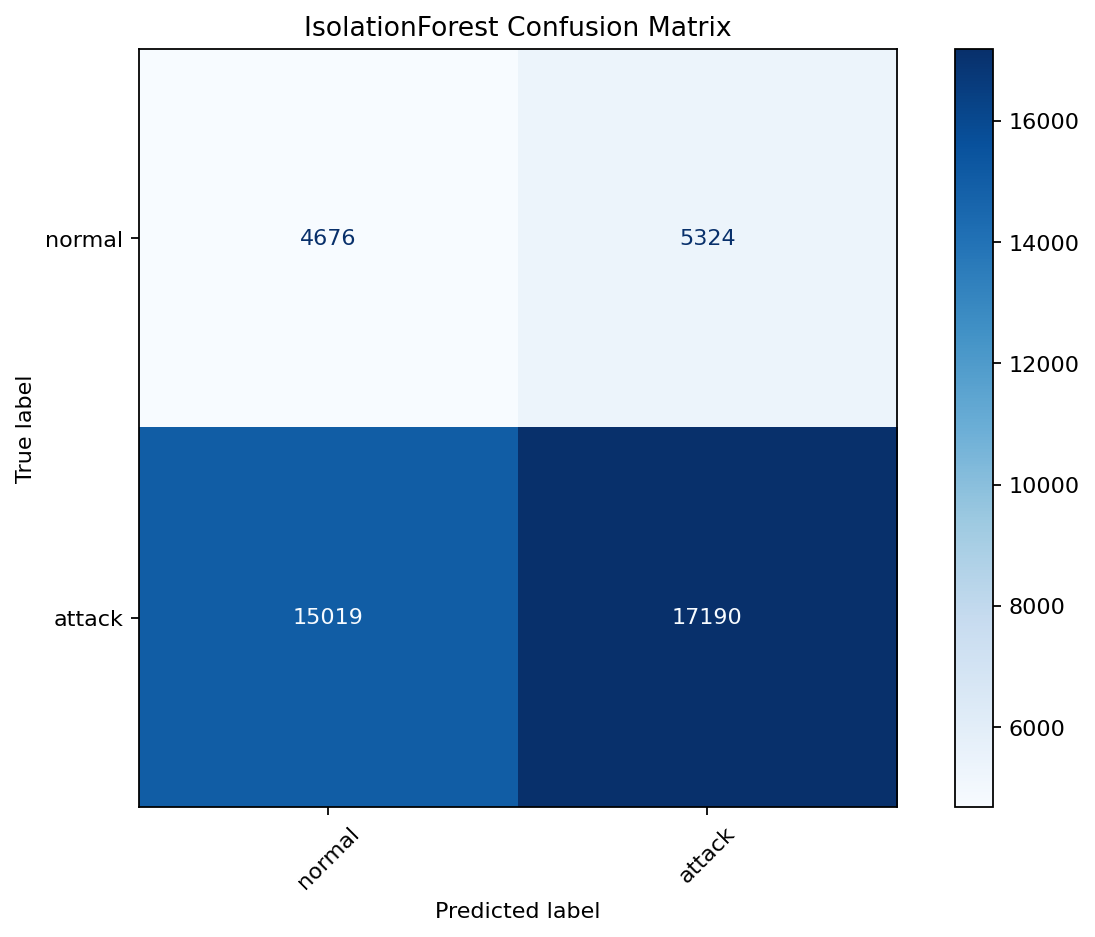
\includegraphics[width=0.95\textwidth]{isolationforest_confusion_matrix.png}
  \caption{IsolationForest Confusion Matrix: Binary anomaly detection (normal vs.~attack)}
  \label{fig:iso-cm}
\end{figure}

RandomForest produces nearly identical results to XGBoost, with both diagonal
dominated patterns indicating few classification errors. IsolationForest, being
unsupervised and binary (normal vs.\ anomaly), cannot differentiate specific
attack types and is reserved for novelty detection in IDS-AI.

\subsection{Example ML Output}

The following example illustrates the runtime output returned by the ML layer
for a suspicious HTTP event. The values are representative of the backend
schema and show how the model result is interpreted by the rest of the
pipeline.

\begin{lstlisting}[style=jsonstyle, caption={Example ML layer output}]
{
  "ml_label": "injection",
  "ml_confidence": 0.987,
  "ml_model": "XGBoost",
  "is_anomaly": true,
  "attack_type": "sql_injection",
  "risk_signals": [
    {"name": "suspicious_http_body", "score": 0.91},
    {"name": "abnormal_request_size", "score": 0.84}
  ],
  "top_features": [
    {"feature": "http_request_body_len", "importance": 0.32},
    {"feature": "src_bytes", "importance": 0.21},
    {"feature": "dst_bytes", "importance": 0.17}
  ]
}
\end{lstlisting}

In this output, \texttt{ml\_label} is the class predicted by the model,
\texttt{ml\_confidence} expresses how sure the model is about that
prediction, and \texttt{is\_anomaly} indicates whether the event should be
treated as suspicious. The \texttt{attack\_type} field gives the predicted
attack family, while \texttt{risk\_signals} and \texttt{top\_features}
explain which patterns pushed the model toward that decision. Together, these
fields give the analyst a fast first-line verdict and a short technical
explanation of why the event was flagged.

\section{LLM Stage}
\label{sec:llm}

When the ML model identifies an anomaly, or when low-confidence web traffic
matches the force-review rule, IDS-AI invokes the LLM layer. The default
provider is Ollama using \texttt{phi3}, and the code also supports a
HuggingFace text-generation pipeline when configured. The LLM is given
sanitized raw log text, ML metadata, risk signals, top features, and selected
knowledge-base context. It returns a structured classification containing:

\begin{itemize}[leftmargin=1.5em]
  \item \texttt{classification}: Normal, Suspicious, or Malicious;
  \item \texttt{attack\_type};
  \item \texttt{severity};
  \item evidence and knowledge-base matches;
  \item explanation;
  \item recommended action;
  \item manual-review flag.
\end{itemize}

\subsection{How the LLM Layer Works}

The LLM receives a tightly controlled prompt constructed from a sanitized
raw log, a compact ML summary (label, confidence, top features, risk signals),
and short snippets selected from \texttt{backend/ml/knowledge\_base.txt}. The
prompt template requires a JSON-only structured reply to make downstream
parsing reliable. The backend enforces length limits and detects
prompt-injection patterns; suspect inputs are redacted before being sent to
the model.

\subsection{Example LLM Output}

The LLM output extends the ML verdict with a human-readable security
assessment. It is especially useful when the model suspects malicious
behaviour and the analyst needs a concise explanation of the incident.

\begin{lstlisting}[style=jsonstyle, caption={Example LLM layer output}]
{
  "classification": "Malicious",
  "attack_type": "sql_injection",
  "severity": "high",
  "llm_confidence": 0.964,
  "evidence": [
    "UNION SELECT pattern detected",
    "Suspicious HTTP payload and body length"
  ],
  "knowledge_matches": [
    "SQL injection often targets HTTP parameters and form fields"
  ],
  "explanation": "The request contains a SQL injection payload and matches known attack behaviour.",
  "recommended_action": "Block the source IP, alert the analyst, and inspect related sessions.",
  "needs_manual_review": true,
  "llm_available": true
}
\end{lstlisting}

In this output, \texttt{classification} is the final natural-language verdict
returned by the LLM, \texttt{severity} summarizes the operational risk, and
\texttt{llm\_confidence} gives the LLM's own confidence estimate. The
\texttt{evidence} and \texttt{knowledge\_matches} fields justify the verdict
with observed indicators and knowledge-base matches, while
\texttt{explanation} and \texttt{recommended\_action} translate the
technical analysis into an actionable message for the security analyst. The
\texttt{needs\_manual\_review} flag makes it explicit when the case should be
reviewed before any response is taken.

Key properties:
\begin{itemize}[leftmargin=1.5em]
  \item Contextual reasoning: the LLM provides human-readable explanations
    and can correlate indicators that the ML layer misses.
  \item Higher latency compared to ML --- calls are executed off the event
    loop through \texttt{asyncio.to\_thread}.
  \item Structured output: classification, evidence items, suggested severity,
    and recommended mitigation steps.
\end{itemize}

\subsection{Safety and Reliability}

To limit misuse and instability the system:
\begin{itemize}[leftmargin=1.5em]
  \item sanitizes and truncates raw logs;
  \item applies prompt-injection detection rules and redaction policies;
  \item limits concurrent LLM execution through the internal
    \texttt{LLMQueue} semaphore;
  \item isolates blocking LLM calls in a background thread when necessary.
\end{itemize}

\section{Prompt Injection Protection}

The backend sanitizes raw logs before sending them to the LLM. It truncates
long input, removes control characters, decodes URL-encoded strings, and
checks for prompt-injection patterns such as instructions to ignore previous
rules, system-role markers, or requests to override the model's behaviour.
If such a pattern is found, the raw log is redacted before LLM analysis.

\section{Final Classification}

The final output combines ML confidence and LLM confidence into a single
result. Anomalies are saved as alerts, while all analyzed events are saved as
traffic records when MongoDB is available.

\section{Human-in-the-Loop Decision Layer}

The final operational decision is not made automatically by the ML model or
the LLM. Instead, IDS-AI follows a Human-in-the-Loop approach. After the ML
layer predicts the traffic label and the LLM layer produces explanations,
evidence, severity, and recommended action, the security analyst reviews the
complete result in the dashboard.

\subsection{How the Human-in-the-Loop Works}

The dashboard aggregates ML outputs, LLM explanations, and persisted traffic
history for each analyzed event. An analyst inspects the combined context and
can change alert workflow status (\texttt{open}, \texttt{reviewing},
\texttt{resolved}, \texttt{false\_positive}) via the UI. Alert records include
timestamps, status, evidence, recommended action, and confidence values so the
review process can be reconstructed from stored data.

\subsection{UX and Operational Recommendations}

Recommended features include:
\begin{itemize}[leftmargin=1.5em]
  \item a dedicated action history log for each alert;
  \item one-click escalation workflows that attach relevant logs to tickets;
  \item role-based access control so only authorized users can resolve alerts.
  \item a future durable analysis job queue if high-volume asynchronous
    processing becomes a production requirement.
\end{itemize}

% ================================================================
\chapter{Database and Persistence}

\section{MongoDB Collections}

The persistence layer stores operational data in MongoDB. The main collections
created by the backend are:

\begin{itemize}[leftmargin=1.5em]
  \item \texttt{alerts}: IDS alerts generated when traffic is classified as
    anomalous.
  \item \texttt{network\_traffic}: analyzed traffic records and classification
    summaries.
  \item \texttt{network\_traffic\_stats}: aggregated traffic counters grouped
    into time windows for dashboard charts.
  \item \texttt{users}: dashboard user accounts and authentication data.
\end{itemize}

\section{Alert Workflow}

Alerts include severity, classification, source and destination IP addresses,
recommended actions, evidence, and workflow status. The dashboard allows an
operator to update alert status using values such as \texttt{open},
\texttt{reviewing}, \texttt{resolved}, and \texttt{false\_positive}.
This workflow represents the Human-in-the-Loop layer: the system provides
analysis, but the analyst decides how the alert should be handled.

\section{Traffic Storage}

Anomalous, suspicious, or malicious analyses are stored as traffic records
with the raw event, model outputs, explanation, evidence, and final
classification. Normal events update the \texttt{network\_traffic\_stats}
collection so the dashboard can still show traffic volume without storing
every benign flow as a full alert-like record.

% ================================================================
\chapter{Frontend Dashboard}

\section{Dashboard Overview}

The frontend is implemented as a React and TypeScript application. The route
configuration lives in \texttt{frontend/src/router/router.tsx}. Protected
dashboard routes include Traffic Monitor, Network Stats, Threats Analysis,
Suggested Actions, Help and Support, Preferences, and Profile pages. API
requests are organized in \texttt{frontend/src/services/}, while React Query
and Zustand manage fetched data and client state.

\section{Traffic View}

The Traffic Monitor view displays persisted network traffic returned by
\texttt{GET /api/traffic}. Rows include:

\begin{itemize}[leftmargin=1.5em]
  \item source and destination addresses;
  \item protocol, service, ports, duration, and packet-size fields;
  \item ML label, anomaly flag, confidence, and severity;
  \item LLM explanation, evidence, risk signals, and recommended action when
    the selected row is opened for detail.
\end{itemize}

\screenshot{traffic\_monitor.png}{Traffic Monitor page with persisted IDS traffic records}

\section{Human Analyst Review}

The dashboard is also the interface for the Human-in-the-Loop layer. It
centralizes ML predictions, LLM explanations, evidence, confidence, severity,
and recommended actions so the analyst can make a final decision with all
available context.

\section{Alerts View}

The Threats Analysis view displays recent IDS alerts, including severity
badges, classification, confidence, evidence, explanation, knowledge matches,
and recommended action. Security analysts can open an alert detail modal and
update the workflow status.

\screenshot{threats\_analysis.png}{Threats Analysis page with severity and status controls}

\section{Network Statistics and Suggestions}

The Network Stats page uses the \texttt{/api/stats} endpoints to show attacks
by type, severity, status, traffic by protocol and service, alerts over time,
top attacker IPs, and top talker IPs. The Suggested Actions page calls
\texttt{/api/suggestions}, groups open alerts by attack type and source IP,
and presents recommended actions derived from the stored LLM analysis.

\section{System Health}

The dashboard can consume \texttt{/api/health} to display the ML model name,
model load status, F1 score, LLM provider and model, LLM enabled/loaded state,
and MongoDB storage connectivity. This makes operational issues visible
without opening backend logs.

% ================================================================
\chapter{Testing and Evaluation}

\section{Training Dataset and Preprocessing}

\subsection{Dataset Source and Size}

The ML model is trained on network flow records loaded from
\texttt{backend/ml/data.csv}. The full dataset contains flow-level features
inspired by Zeek and CTU datasets. Each row represents a single network flow
and includes TCP/UDP statistics, HTTP metadata, DNS queries, and a label
indicating the attack type or normal classification.

The complete dataset contains over 40,000 network flows across 10 attack
classes plus normal traffic. These are split into:

\begin{itemize}[leftmargin=1.5em]
  \item \textbf{Training set (80\%):} Approximately 32,000 flows used to fit
    the model parameters, class encoders, and feature scalers.
  \item \textbf{Test set (20\%):} Approximately 8,000 flows held back to
    evaluate final model performance without any data leakage.
\end{itemize}

Stratified splitting is used to preserve class proportions in both splits,
ensuring the test set reflects the real-world class imbalance.

\subsection{Feature Engineering}

The model operates on 20 numeric features and 3 categorical features:

\begin{itemize}[leftmargin=1.5em]
  \item \textbf{Numeric features:} \texttt{src\_port, dst\_port, duration,
    src\_bytes, dst\_bytes, missed\_bytes, src\_pkts, src\_ip\_bytes,
    dst\_pkts, dst\_ip\_bytes, dns\_qclass, dns\_qtype, dns\_rcode,
    http\_request\_body\_len, http\_response\_body\_len, http\_status\_code,
    http\_trans\_depth}.
  \item \textbf{Categorical features:} \texttt{proto} (TCP, UDP, ICMP),
    \texttt{service} (HTTP, FTP, SSH, DNS, etc.), \texttt{conn\_state}
    (connection state codes).
\end{itemize}

Numeric features are standardized to zero mean and unit variance using a
\texttt{StandardScaler} fitted on the training set. Categorical features are
ordinal-encoded using \texttt{LabelEncoder}. Missing numeric values are
imputed as zero; unknown categorical values are mapped to $-1$.

\subsection{Class Distribution and Imbalance}

Table~\ref{tab:class-distribution} summarizes the attack type distribution
in the full dataset before any augmentation:

\begin{table}[htbp]
  \centering
  \caption{Attack type distribution in full training dataset (before SMOTE)}
  \label{tab:class-distribution}
  \begin{tabular}{lrr}
    \toprule
    \textbf{Attack Type} & \textbf{Count} & \textbf{Percentage} \\
    \midrule
    normal      & 13000 & 32.3\% \\
    ddos        & 8000  & 19.9\% \\
    dos         & 7800  & 19.4\% \\
    backdoor    & 4000  & 10.0\% \\
    ransomware  & 2000  & 5.0\% \\
    injection   & 2000  & 5.0\% \\
    password    & 1000  & 2.5\% \\
    xss         & 1000  & 2.5\% \\
    scanning    & 1000  & 2.5\% \\
    mitm        & 200   & 0.5\% \\
    \midrule
    \textbf{Total} & \textbf{40000} & \textbf{100\%} \\
    \bottomrule
  \end{tabular}
\end{table}

The dataset exhibits significant class imbalance: MITM represents only 0.5\%
of samples while normal traffic represents 32.3\%. Without correction, the
model would overfit to majority classes and fail to detect rare attack types.

\subsection{SMOTE Augmentation on Training Set}

To mitigate class imbalance, SMOTE (Synthetic Minority Over-sampling Technique)
is applied exclusively to the training set. SMOTE generates synthetic samples
by interpolating between minority class samples and their $k=5$ nearest
neighbors in feature space. The sampling strategy is set to
\texttt{``not\_majority''}, meaning all attack types are upsampled to match
the size of the most frequent attack class within the training split.

Example augmentation results from one training run:

\begin{table}[htbp]
  \centering
  \caption{Dataset size growth due to SMOTE augmentation (training set only)}
  \label{tab:smote-augmentation}
  \begin{tabular}{lrrr}
    \toprule
    \textbf{Phase} & \textbf{Dataset Size} & \textbf{Normal:Attack Ratio} & \textbf{Note} \\
    \midrule
    Original training split & 32,000 & 2.4:1 & Before SMOTE \\
    After SMOTE            & 48,000 & 1.3:1 & Synthetic samples added \\
    \bottomrule
  \end{tabular}
\end{table}

By increasing the training set from 32,000 to 48,000 samples with balanced
attack class representation, the model learns discriminative features for all
attack types without being overwhelmed by normal traffic. Importantly, SMOTE
is \textbf{not} applied to the test set, keeping it genuinely imbalanced and
realistic for unbiased evaluation.

\section{Synthetic Attack Dataset for API Testing}

The project includes a generated synthetic intrusion dataset for load testing:
\texttt{load\_tests/synthetic\_intrusion\_dataset\_450.json}. It contains 450
events: 25 entries for each of 18 labels. The labels are:

\begin{center}
\begin{tabular}{llll}
\toprule
normal & backdoor & ddos & dos \\
injection & portscan & nmap & ipsweep \\
ftp\_write & guess\_passwd & buffer\_overflow & neptune \\
smurf & teardrop & bruteforce & xss \\
sql\_injection & botnet & & \\
\bottomrule
\end{tabular}
\end{center}

Each record follows the same JSON schema as the backend \texttt{LogEvent}
model. Normal records use benign user IP addresses from
\texttt{192.168.1.0/24}, while attack records use source addresses from
\texttt{198.51.100.0/24}. Target hosts use \texttt{10.0.0.0/24}. This dataset
is used for API-level detection tests and demonstration traffic, not for model
training.

\section{Attack Request Test}

The file \texttt{load\_tests/run\_attack\_queue\_test.py} generates and
submits 100 attack events to the backend. The script writes
\texttt{attack\_requests\_100.json} and can be adapted to post each entry to
\texttt{/api/analyze}. Since the current public API does not expose
\texttt{/api/analysis/jobs}, this script should be treated as a load-test
utility that must stay synchronized with the backend route design.

\begin{lstlisting}[style=bashstyle, caption={Running the attack request test utility}]
python3 load_tests/run_attack_queue_test.py \
  --api-base http://127.0.0.1:8001 \
  --wait-seconds 60
\end{lstlisting}

\section{Expected Test Result}

When pointed at the implemented \texttt{/api/analyze} endpoint, attack samples
should produce ML labels such as \texttt{ddos}, \texttt{dos},
\texttt{injection}, \texttt{xss}, \texttt{backdoor}, or related attack
families. Samples that are anomalous or force-reviewed should also receive
LLM evidence, an explanation, a recommended action, and
\texttt{needs\_manual\_review=true}. Alerts should be saved in MongoDB when
storage is enabled.

\begin{table}[htbp]
  \centering
  \caption{Expected fields for attack API validation}
  \label{tab:attack-api-result}
  \begin{tabular}{ll}
    \toprule
    \textbf{Field} & \textbf{Expected Behaviour} \\
    \midrule
    \texttt{is\_anomaly} & \texttt{true} for generated attack samples \\
    \texttt{classification} & \texttt{Suspicious} or \texttt{Malicious} \\
    \texttt{severity} & \texttt{medium} or \texttt{high} for confirmed attacks \\
    \texttt{evidence} & Payload, traffic, or knowledge-base indicators \\
    \texttt{recommended\_action} & Analyst-facing response step \\
    \bottomrule
  \end{tabular}
\end{table}

This validation confirms the behaviour of the implemented ML + LLM path. A
separate public asynchronous queue would be a future improvement rather than
part of the current backend contract.

\section{Build Verification}

\begin{lstlisting}[style=bashstyle, caption={Verification commands}]
python3 -m py_compile backend/main.py backend/router/analyse/analyse.py \
  backend/schemas/schemas.py
npm run build
\end{lstlisting}

The expected verification checks are Python syntax compilation for the backend
and a TypeScript/Vite production build for the frontend.

% ================================================================
\chapter{Security Considerations}

\section{Local LLM Deployment}

Using Ollama keeps LLM processing local, which avoids sending sensitive raw
network logs to external cloud services. This is important because intrusion
logs may contain IP addresses, internal paths, request bodies, or other
security-sensitive metadata.

\section{Input Sanitization}

Raw logs are treated as untrusted data. The backend truncates and sanitizes
raw input before it is used in an LLM prompt. Prompt-injection detection
reduces the risk of malicious traffic logs manipulating the LLM.

\section{LLM Concurrency Protection}

The internal LLM queue uses a semaphore to limit concurrent LLM calls. This is
important because local LLM inference can consume significant CPU, GPU, and
memory resources. The current code serializes LLM calls with
\texttt{max\_concurrent=1}.

\section{Operational Limitations}

The synchronous \texttt{/api/analyze} endpoint is suitable for demonstration
and controlled testing. For production use, a durable external queue such as
Redis, RabbitMQ, or Kafka would be recommended so large bursts of analysis
requests can survive process restarts and be distributed across multiple
workers or machines.

% ================================================================
\chapter{Conclusion}

IDS-AI demonstrates a practical three-layer approach to intrusion detection.
The machine learning model provides fast classification from structured
network features, the LLM adds interpretability, evidence, and recommended
actions for suspicious or malicious events, and the Human-in-the-Loop layer
keeps the final decision under analyst control. The FastAPI backend, MongoDB
persistence layer, and React dashboard work together to provide both analysis
and operational visibility.

The most important architectural choice is the hybrid analysis flow. The ML
detector produces fast predictions, payload inspection catches obvious
injection patterns even when the model predicts normal, and the LLM layer adds
structured explanations when deeper review is needed. The dashboard then
turns those outputs into alert review, network statistics, and suggested
actions.

Future improvements could include a durable distributed queue with public job
status endpoints, stronger role-based dashboard access, richer model metrics,
automated report export for incident response, and tighter integration between
WebSocket updates and the traffic/alert tables.

% ================================================================
\appendix

\chapter{Environment Variables}

\begin{lstlisting}[style=bashstyle, caption={Recommended backend environment variables}]
LLM_PROVIDER=ollama
LLM_MODEL_NAME=phi3
OLLAMA_BASE_URL=http://localhost:11434
LLM_ENABLED=true
MONGO_ENABLED=true
MONGO_URI=mongodb://localhost:27017/ids_ai
DATABASE_NAME=ids_ai
CORS_ORIGINS=http://localhost:5173
IDS_MODEL_PATH=backend/ml/best_model.joblib
LLM_PRELOAD=false
\end{lstlisting}

\chapter{Example API Response}

\begin{lstlisting}[style=jsonstyle, caption={Example completed analysis result}]
{
  "timestamp": "2026-05-01T12:00:00Z",
  "ml_label": "injection",
  "ml_confidence": 0.88,
  "ml_model": "XGBoost",
  "is_anomaly": true,
  "attack_type": "injection",
  "classification": "Malicious",
  "llm_attack_type": "sql_injection",
  "llm_severity": "critical",
  "llm_confidence": 0.92,
  "evidence": ["UNION SELECT pattern detected"],
  "knowledge_matches": ["SQL Injection"],
  "explanation": "The HTTP payload contains SQL injection indicators.",
  "recommended_action": "Block the source IP and inspect web server logs.",
  "needs_manual_review": true,
  "llm_available": true,
  "final_confidence": 0.89,
  "severity": "high",
  "src_ip": "198.51.100.10",
  "dst_ip": "10.0.0.20",
  "src_port": 20000,
  "dst_port": 80,
  "protocol": "tcp",
  "service": "http"
}
\end{lstlisting}

\end{document}
